\subsection{State space representation}\label{chapter_StateSpaceIMPL}

As mentioned in the chapter \ref{chapter_Approach}, first step in developing the state space controller is, to analyze the process of the quadrocopter. This process is introduced and explained in chapter \ref{chapter_DYNAMICS_BLOCK}. Chapter \ref{chapter_StateSpace} explains the basic knowledge about state space representation, needed in this chapter. Figure \ref{fig:MATLAB Dynamics Sections} shows the process of the quadrocopter. 

First of all it is necessary to find out, which part of the process is really needed to control the quadrocopter. So the earthframe part (blue) of the quadrocopter can be eliminated. 
Figures \ref{fig:MATLAB Dynamics1} and \ref{fig:MATLAB Dynamics2} are showing, how the remain looks like. That is only the bodyframe part of the process. And this part, is that one, the state space controller has to deal with.

\subsubsection{Controllability}\label{chapter_controllabilityIMPL}

Now the part of the process, that has to be controlled, is filtered out. Next step is, to check whether the process is controllable or not. To do so, the rank of the controllability matrix has to be the same as the number of state variables in the process. The easiest way to prove the controllability is, to use the ctrb() command in MATLAB. It returns the rank of the controllability matrix, which has to be compared with the number of state variables. With the linmod() function, it is possible to get the state space matrices of a Simulink model. 

Like figures \ref{fig:MATLAB Dynamics1} and \ref{fig:MATLAB Dynamics2} are showing, there are nine state variables that have to be controlled. These nine state variables, are the four motor delays (\ref{chapter_GREEN_SECTION}), the rate and the angle of phi, the rate and the angle of theta and the rate of psi. The angle of psi is not important, because it need not be controlled.

\begin{lstlisting}
	System = linmod('dynamics_reduced');
	StateSpace = ss(System.a, System.b, System.c, System.d);
	rank(ctrb(StateSpace))  
	% ans = 4                 
\end{lstlisting}

As the code snippet reveals, only four of the nine state variables can be controlled. Now there are two options to choose from. One is, to cancel the development process of the state space controller. But that is not the engineers way. The other option is, to continue reducing the model to gain full controllability. The next section deals with that.

\subsubsection{Model reduction}\label{chapter_ModelReductionIMPL}

The already reduced process without the earthframe part, is not controllable (chapter \ref{chapter_controllabilityIMPL}). So there is need to reduce the model once again, but all remaining parts of the model are needed to construct the state space controller. In this stage, the reduced process has to be examined very carefully. Looking at the delay in the four motors of the process, reveals, that there is only one millisecond delay in each motor (figure \ref{fig:motorWithDelay}).

\begin{figure}
	\centering
		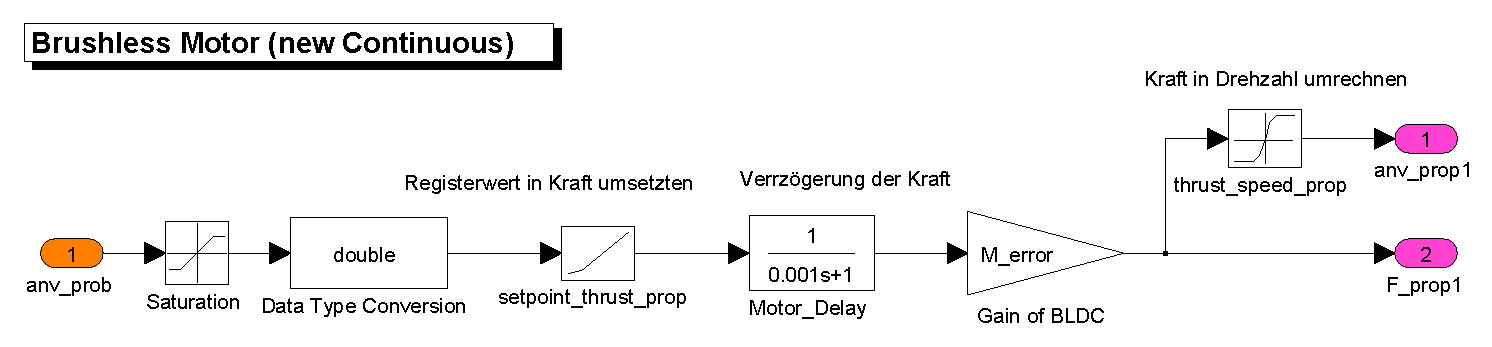
\includegraphics[width=1.00\textwidth]{03_Grafiken/motorWithDelay.pdf}
	\caption{Model of one motor including the time delay}
	\label{fig:motorWithDelay}
\end{figure}

In comprehension to the delays in each of the processes remaining integrators, the one millisecond can be disregarded (figure \ref{fig:motorWithoutDelay}). Now the same code, already used in chapter \ref{chapter_controllabilityIMPL}, has to run again, to check the controllability.

\begin{figure}
	\centering
		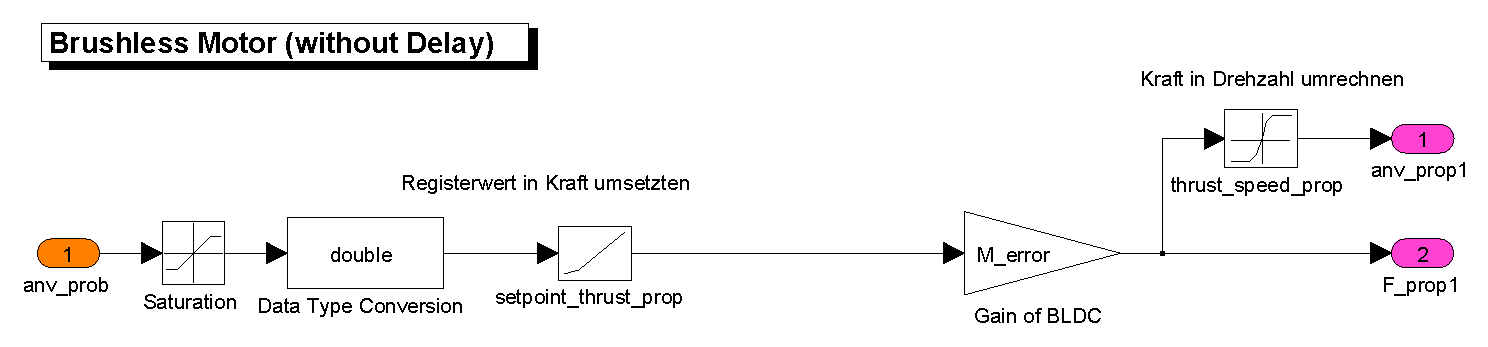
\includegraphics[width=1.00\textwidth]{03_Grafiken/motorWithoutDelay.pdf}
	\caption{Model of one motor without the time delay}		
	\label{fig:motorWithoutDelay}
\end{figure}


\begin{lstlisting}
	System = linmod('dynamics_reduced_without_motordelay');
	StateSpace = ss(System.a, System.b, System.c, System.d);
	rank(ctrb(StateSpace))  
	% ans = 5                 
\end{lstlisting}

Now the rank of the controllability matrix is five. That is the right number of controllable state variables, because the four motor delays are removed and so there are only five state variables remaining. At this point of the development it is not sure, if the state space controller, developed for this model without motor delay, will work later on with the process including the motor delay.


\subsubsection{Observability}\label{chapter_observabilityIMPL}

Just a few words about the observability of the process. Five states are controllable - the rate of phi, theta, psi and the angle of phi and theta. Chapter \ref{chapter_SENSORS} shows the sensors, used in the quadrocopter. For each of the five state variables there is a sensor. That is the reason, why no observer is needed in this project, but - maybe interesting for a further project - the observability of the system is given. So it might be possible to reduce the number of sensors and develop an observer instead. The following code snippet shows that.

\begin{lstlisting}
	System = linmod('dynamics_reduced_without_motordelay');
	StateSpace = ss(System.a, System.b, System.c, System.d);
	rank(obsv(StateSpace)) 
	% ans = 5                 
\end{lstlisting}
